% ----------------------------------------------------------
\chapter{Comandos do \LaTeX, do \abnTeX\ e do UnB\TeX}
\label{cap_exemplos}
% ----------------------------------------------------------

Este capítulo ilustra o uso de comandos do \LaTeX, do \abnTeX\ e do UnB\TeX. 

% ---
\section{Codificação dos arquivos: UTF8}
% ---

A codificação de todos os arquivos do \abnTeX\ é \texttt{UTF8}. É necessário que você utilize a mesma codificação nos documentos que escrever, inclusive nos arquivos de base bibliográficas \verb|.bib|.

% ---
\section{Citações diretas}\label{sec-citacao}
% ---

Utilize o ambiente \texttt{citacao} para incluir citações diretas com mais de três linhas:

\begin{citacao}
As citações diretas, no texto, com mais de três linhas, devem ser destacadas com recuo de 4 cm da margem esquerda, com letra menor que a do texto utilizado e sem as aspas. No caso de documentos datilografados, deve-se observar apenas o recuo \cite[seção 5.3]{NBR10520:2002}.
\end{citacao}

Use o ambiente assim:

\begin{verbatim}
\begin{citacao}
As citações diretas, no texto, com mais de três linhas [...] deve-se observar
apenas o recuo \cite[seção 5.3]{NBR10520:2002}.
\end{citacao}
\end{verbatim}

O ambiente \texttt{citacao} pode receber como parâmetro opcional um nome de idioma previamente carregado nas opções da classe (\cref{sec-hifenizacao}). Nesse caso, o texto da citação é automaticamente escrito em itálico e a hifenização é ajustada para o idioma selecionado na opção do ambiente. Por exemplo:

\begin{verbatim}
\begin{citacao}[english]
Text in English language in italic with correct hyphenation.
\end{citacao}
\end{verbatim}

Tem como resultado:

\begin{citacao}[english]
Text in English language in italic with correct hyphenation.
\end{citacao}

Citações simples, com até três linhas, devem ser incluídas com aspas. Observe que em \LaTeX\ as aspas iniciais são diferentes das finais: ``Amor é fogo que arde sem se ver''.

% ---
\section{Notas de rodapé}
% ---

As notas de rodapé são detalhadas pela NBR 14724:2011 na seção 5.2.1\footnote{As notas devem ser digitadas ou datilografadas dentro das margens, ficando separadas do texto por um espaço simples de entre as linhas e por filete de 5 cm, a partir da margem esquerda. Devem ser alinhadas, a partir da segunda linha da mesma nota, abaixo da primeira letra da primeira palavra, de forma a destacar o expoente, sem espaço entre elas e com fonte menor \citeonline[seção 5.2.1]{NBR14724:2011}.}\footnote{Caso uma série de notas sejam criadas sequencialmente, o \abnTeX\ instrui o \LaTeX\ para que uma vírgula seja colocada após cada número do expoente que indica a nota de rodapé no corpo do texto.}\footnote{Verifique se os números do expoente possuem uma vírgula para dividi-los no corpo do texto.}.

% ---
\section{Tabelas}
% ---

A \cref{tab-nivinv} é um exemplo de tabela construída em
\LaTeX.

\begin{table}[htb]
\footnotesize
\caption[Níveis de investigação]{Níveis de investigação.}
\label{tab-nivinv}
\begin{tabular}{p{2.6cm}|p{6.0cm}|p{2.25cm}|p{3.40cm}}
  %\hline
   \textbf{Nível de Investigação} & \textbf{Insumos}  & \textbf{Sistemas de Investigação}  & \textbf{Produtos}  \\
    \hline
    Meta-nível & Filosofia da Ciência  & Epistemologia &
    Paradigma  \\
    \hline
    Nível do objeto & Paradigmas do metanível e evidências do nível inferior &
    Ciência  & Teorias e modelos \\
    \hline
    Nível inferior & Modelos e métodos do nível do objeto e problemas do nível inferior & Prática & Solução de problemas  \\
   % \hline
\end{tabular}
\legend{Fonte: \citeonline{van86}}
\end{table}

Já a \cref{tabela-ibge} apresenta uma tabela criada conforme o padrão do \citeonline{ibge1993} requerido pelas normas da ABNT para documentos técnicos e acadêmicos.

\begin{table}[htb]
\IBGEtab{%
  \caption{Um Exemplo de tabela alinhada que pode ser longa
  ou curta, conforme padrão IBGE.}%
  \label{tabela-ibge}
}{%
  \begin{tabular}{ccc}
  \toprule
   Nome & Nascimento & Documento \\
  \midrule \midrule
   Maria da Silva & 11/11/1111 & 111.111.111-11 \\
  \midrule 
   João Souza & 11/11/2111 & 211.111.111-11 \\
  \midrule 
   Laura Vicuña & 05/04/1891 & 3111.111.111-11 \\
  \bottomrule
\end{tabular}%
}{%
  \fonte{Produzido pelos autores.}%
  \nota{Esta é uma nota, que diz que os dados são baseados na   regressão linear.}%
  \nota[Anotações]{Uma anotação adicional, que pode ser seguida de várias outras.}%
  }
\end{table}

Na \cref{tab:lvlii} são mostrados os componentes curriculares do novo fluxograma da engenharia mecatrônica.

\begin{table}[htb]
\small
\begin{center}%
\caption{Componentes curriculares do segundo nível} \label{tab:lvlii}
\noindent%
\begin{tabular}{|m{1.5cm}|m{4.3cm}|m{.7cm}|m{.7cm}|m{.7cm}|m{.7cm}|m{.7cm}|m{2.1cm}|}
\hline%
\multicolumn{8}{|l|}{\textbf{2º Nível}} \\\hline%
\multirow{2}{*}{Código} &
\multirow{2}{*}{Componente curricular} &
\multicolumn{5}{c|}{Quantidade de horas} & 
\multirow{2}{*}{Pré-requisito} \\ 
\cline{3-7} & & Teo. & Pr. & Ext. & EaD & Tot. & \\\hline\hline%
MAT0026 & Cálculo 2 & 60 & 30 & 0 & 0 & 90 & MAT0025 \\\hline%
IFD0171 & Física 1 & 60 & 0 & 0 & 0 & 60 & \\\hline%
IFD0173 & Física 1 Experimental & 0 & 30 & 0 & 0 & 30 & \\\hline%
EST0023 & Probabilidade e Estatística & 30 & 30 & 0 & 0 & 60 & MAT0025 \\\hline%
ENM0190 & Desenho Mecânico para Engenharia & 30 & 30 & 0 & 0 & 60 & \\\hline%	
CIC0090 & Estruturas de Dados & 30 & 30 & 0 & 0 & 60 & CIC0004 \\\hline%
\multicolumn{2}{|l|}{Componentes optativos ou eletivos} & & & & & 60 & \multicolumn{1}{r}{} \\\cline{1-7}%
\multicolumn{6}{|l|}{Total de horas do 2º Nível} & 420 & \multicolumn{1}{r}{} \\\cline{1-7}%
\end{tabular}
\end{center}%
\end{table}

É uma boa ideia usar o pacote \textsf{longtable} para criar tabelas, pois assim uma mesma tabela pode ocupar várias páginas. Também há pacotes que rotacionam tabelas, para que fiquem em uma página em formato paisagem. Faça as tabelas usando como base qualquer um dos exemplos aqui apresentados ou outros que considerar mais adequados e que podem ser facilmente encontrados na internet.

% ---
\section{Figuras}
% ---

Existem pacotes que permitem criar figuras e gráficos no próprio código \LaTeX. Por exemplo, temos

\begin{itemize}
    \item PGFPlots \url{http://pgfplots.sourceforge.net/}
    \item TikZ \url{http://www.texample.net/tikz/examples/all/}
    \item Metapost \url{http://tex.loria.fr/prod-graph/zoonekynd/metapost/metapost.html}
    \item PSTricks \url{https://tug.org/PSTricks/main.cgi?file=examples}
\end{itemize}

Figuras também podem ser incorporadas de arquivos externos, como é o caso das \cref{fig_blockdiagram,fig_grafico}. Se a figura que for incluída se tratar de um diagrama, um gráfico ou uma ilustração que você mesmo produza, priorize o uso de imagens vetoriais no formato PDF. Com isso, o tamanho do arquivo final do trabalho será menor, e as imagens terão uma apresentação melhor, principalmente quando impressas, uma vez que imagens vetoriais são perfeitamente escaláveis para qualquer dimensão. Nesse caso, se for utilizar o Microsoft Excel para produzir gráficos, ou o Microsoft Word para produzir ilustrações, exporte-os como PDF e os incorpore ao documento conforme o exemplo abaixo. No entanto, para manter a coerência no uso de software livre (já que você está usando \LaTeX\ e \abnTeX), teste a ferramenta \textsf{InkScape} (\url{http://inkscape.org/}). Ela é uma excelente opção de código-livre para produzir ilustrações vetoriais, similar ao CorelDraw ou ao Adobe Illustrator. De todo modo, caso não seja possível utilizar arquivos de imagens como PDF, utilize qualquer outro formato, como JPEG, GIF, BMP, etc. Nesse caso, você pode tentar aprimorar as imagens incorporadas com o software livre \textsf{Gimp} (\url{http://www.gimp.org/}). Ele é uma alternativa livre ao Adobe Photoshop.

\begin{figure}[htb]
    \centering
    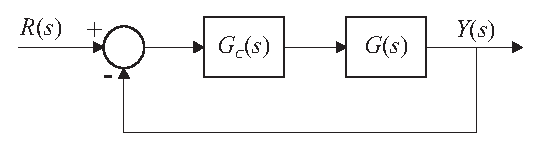
\includegraphics[scale=1]{blockdiagram.eps}
	\caption{\label{fig_blockdiagram}Sistema de controle em malha fechada}
\end{figure}

\begin{figure}[htb]
	\begin{center}
	    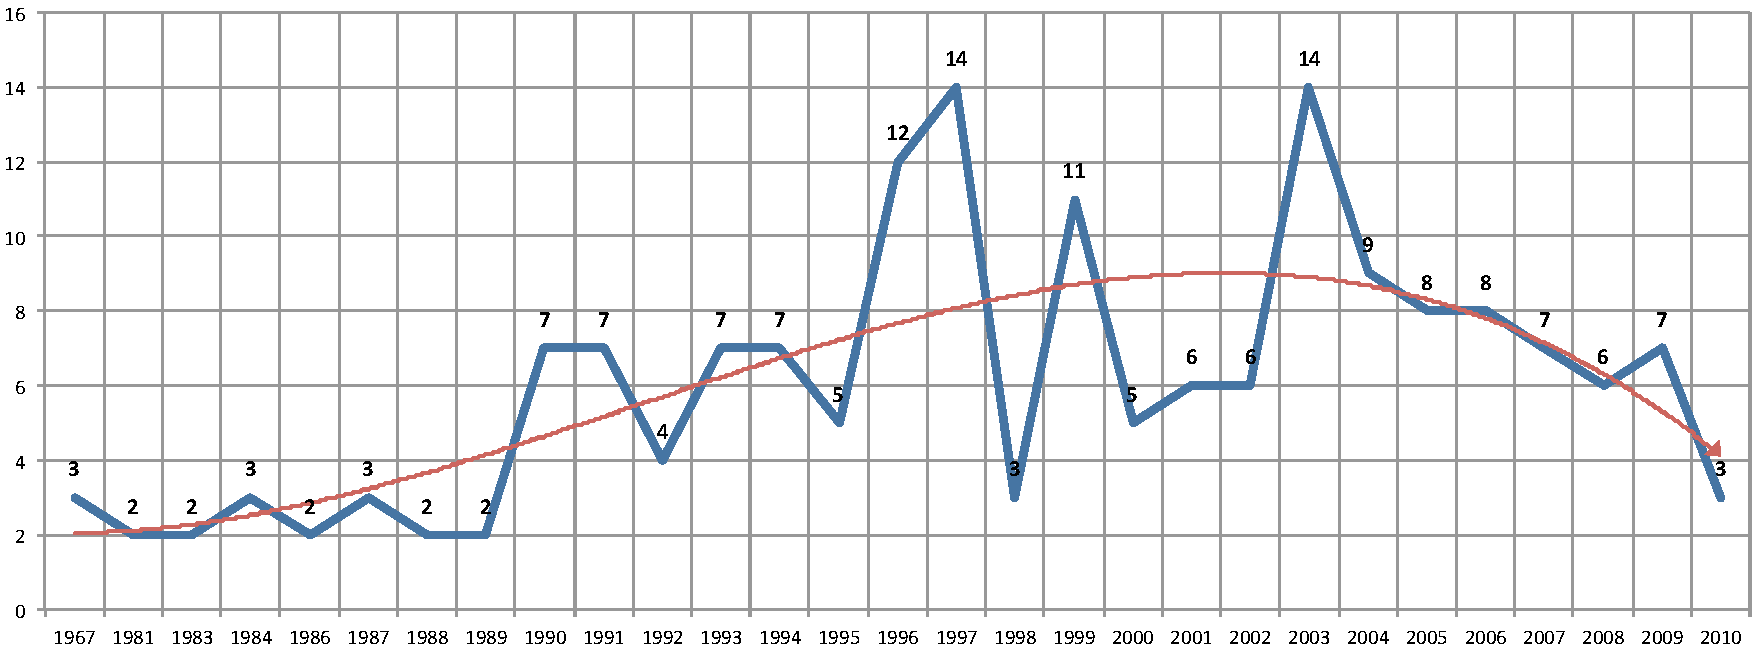
\includegraphics[scale=0.5]{img-grafico.pdf}
	\end{center}
	\caption{\label{fig_grafico}Gráfico produzido em Excel e salvo como PDF}
	\legend{Fonte: \citeonline[24]{araujo2012}}
\end{figure}

% ---
\subsection{Figuras em \emph{minipages}}
% ---

\emph{Minipages} são usadas para inserir textos ou outros elementos em quadros com tamanhos e posições controladas. Veja os exemplos das \cref{fig_minipage_imagem1,fig_minipage_grafico2}.

\begin{figure}[htb]
 \label{teste}
 \centering
  \begin{minipage}{0.4\textwidth}
    \centering
    
\includegraphics[scale=0.9]{img-marca.pdf}
    \caption{Imagem 1 da minipage} \label{fig_minipage_imagem1}
    \legend{Fonte: Produzido pelos autores}
  \end{minipage}
  \hfill
  \begin{minipage}{0.4\textwidth}
    \centering
    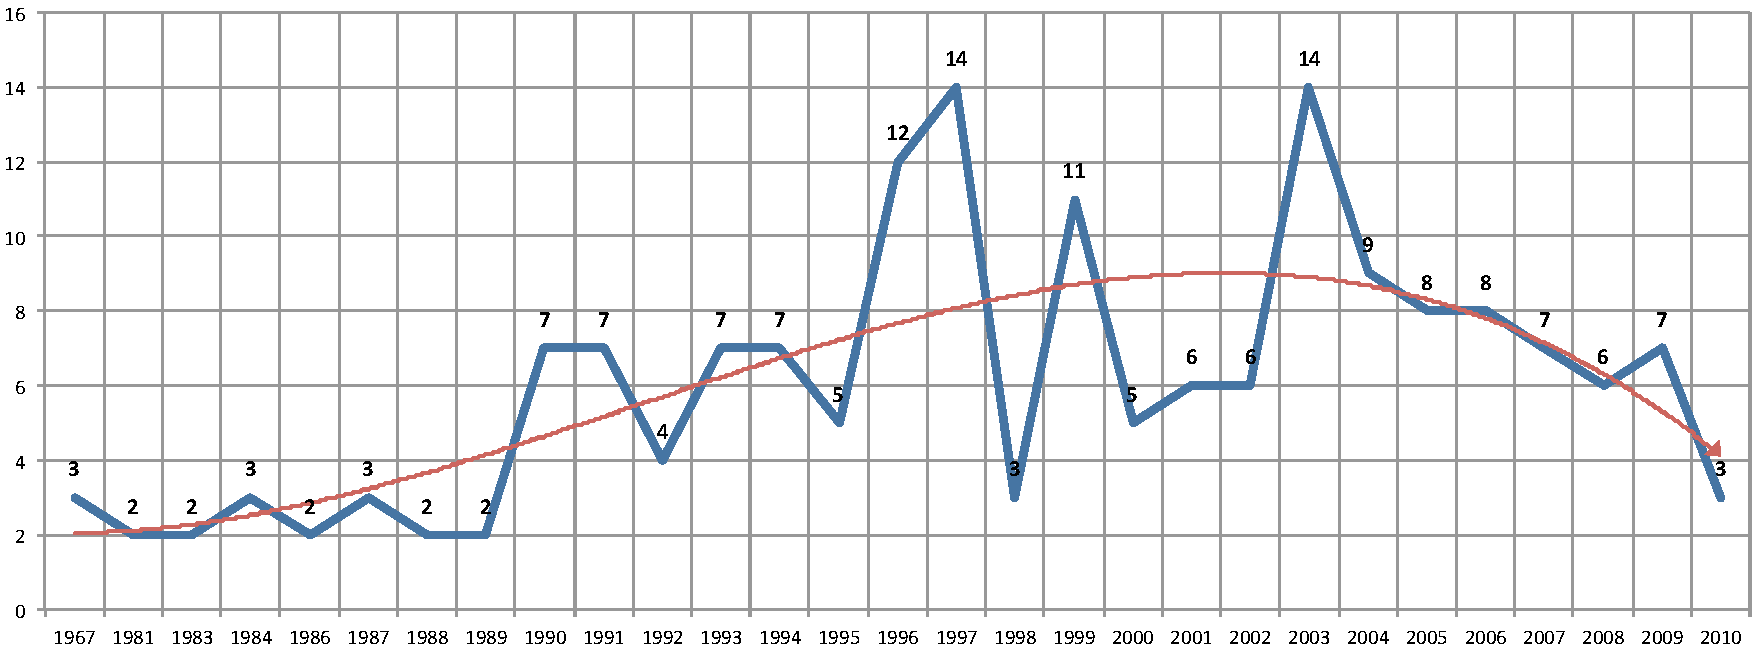
\includegraphics[scale=0.2]{img-grafico.pdf}
    \caption{Gráfico 2 da minipage} \label{fig_minipage_grafico2}
    \legend{Fonte: \citeonline[24]{araujo2012}}
  \end{minipage}
\end{figure}

\subsection{Subfiguras}

\begin{figure}[H]
    \centering
	\begin{subfigure}[t]{0.4\columnwidth}
		
\includegraphics[scale=0.9]{img-marca.pdf}
		\caption{Primeira subfigura}
		\label{fig_subfigura_imagem1}
    \end{subfigure}%
    \hfill
    \begin{subfigure}[t]{0.4\columnwidth}
		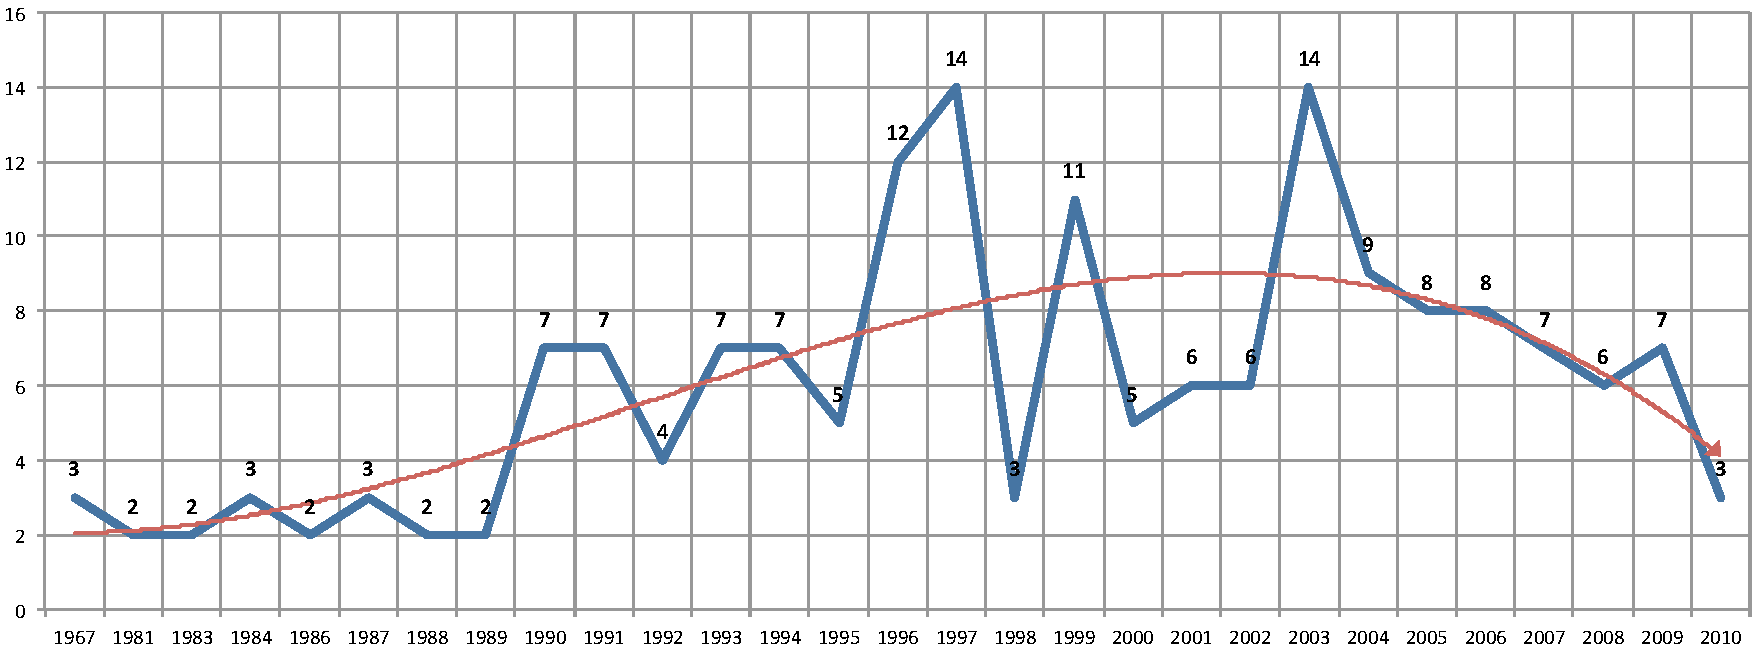
\includegraphics[scale=0.2]{img-grafico.pdf}
		\caption{Segunda subfigura}
		\label{fig_subfigura_grafico2}
    \end{subfigure}
    \caption{Figura com subfiguras}
    \label{fig:tau}
\end{figure}

Observe que, segundo a \citeonline[seções 4.2.1.10 e 5.8]{NBR14724:2011}, as ilustrações devem sempre ter numeração contínua e única em todo o documento:

\begin{citacao}
Qualquer que seja o tipo de ilustração, sua identificação aparece na parte superior, precedida da palavra designativa (desenho, esquema, fluxograma, fotografia, gráfico, mapa, organograma, planta, quadro, retrato, figura, imagem, entre outros), seguida de seu número de ordem de ocorrência no texto, em algarismos arábicos, travessão e do respectivo título. Após a ilustração, na parte inferior, indicar a fonte consultada (elemento obrigatório, mesmo que seja produção do próprio autor), legenda, notas e outras informações necessárias à sua compreensão (se houver). A ilustração deve ser citada no texto e inserida o mais próximo possível do trecho a que se refere. \cite[seção 5.8]{NBR14724:2011}
\end{citacao}

% ---
\section{Expressões matemáticas}
\label{sec-mat}
% ---

Use o ambiente \texttt{equation} para escrever expressões matemáticas numeradas:

\begin{equation}
  \forall x \in X, \quad \exists \: y \leq \epsilon
\end{equation}

Escreva expressões matemáticas entre \$ e \$, como em $ \lim_{x \to \infty} \exp(-x) = 0 $, para que fiquem na mesma linha.

Também é possível usar colchetes para indicar o início de uma expressão matemática que não é numerada.

\[
\left|\sum_{i=1}^n a_ib_i\right|
\le
\left(\sum_{i=1}^n a_i^2\right)^{1/2}
\left(\sum_{i=1}^n b_i^2\right)^{1/2}
\]

Consulte mais informações sobre expressões matemáticas em \url{https://github.com/abntex/abntex2/wiki/Referencias}.

Muitos cientistas gostam de usar \LaTeX\ porque essa ferramenta possibilita escrever facilmente equações como a seguinte:

\begin{equation}
p+\frac{1}{2}{\rho}v^2+{\rho}gh = \text{constante},
 \label{eq:Bernoulli}
\end{equation}

\noindent em que $p$ é a pressão, $v$ é a velocidade e $h$ é a elevação, ou seja, a ``altura do tubo''. A \cref{eq:Bernoulli} pode ser deduzida a partir do \textit{Teorema Trabalho-Energia}.

% Definição da nomenclatura que irá para a lista de símbolos
\nomenclature[B]{$p$}{Pressão}
\nomenclature[B]{$v$}{Velocidade}
\nomenclature[B]{$h$}{Elevação}

A seguir, são apresentados mais alguns exemplos de equações feitas com o \LaTeX.

\newcommand{\vt}[1]{\mathbf{#1}}

\begin{equation}\label{eq:R_f_usual}
\vt{R}_r(t) = \vt{R}_{\chi}(t) \triangleq 
\begin{bmatrix}
\cos \chi_0 (t) & -\sin \chi_0 (t) & 0
\\
\sin \chi_0 (t) & \cos \chi_0 (t) & 0
\\
0 & 0 & 1
\end{bmatrix}
\end{equation}

\begin{equation}
\vt{L}_{ij} = 
\begin{cases}
-a_{ij}, & \text{se } j \neq i \text{ e } j \in \mathcal{N}_i, \\
\sum_{k \in \mathcal{N}_i} a_{ik}, & \text{se } j = i,  \\
0, & \text{caso contrário}.
\end{cases}
\end{equation}

\begin{align}
\tau_{li}^s(t) &= \ddot{p}^d_{li}(t) - k_{d} \dot{e}_{li}(t) - k_{p} e_{li}(t),
\\
\dot{\tau}_{li}^f(t) +  \xi_{i} \tau_{li}^f(t) &= u_{li}(t),\label{eq:filtro_i}
\\
u_{li}(t) &= - \textrm{sign}(s_{li}(t))\eta. \label{eq:u_xbi}
\end{align}

\begin{equation}\label{eq:point-mass-velocity}
\begin{split}
\dot{V}_i(t) &{}= \frac{T_i(t) - D_i(t)}{m_i} - g \sin \gamma_i(t) + b_{ti}(t), \\
\dot{\chi}_i(t) &{}= \frac{L_i(t) \sin \phi_i(t)}{m_i V_i(t) \cos \gamma_i(t)} + \frac{b_{\psi i}(t)}{V_i(t)\cos \gamma_i(t)},\\
\dot{\gamma}_i(t) &{}= \frac{L_i(t) \cos \phi_i(t)}{m_i V_i(t)} - \frac{g \cos \gamma_i(t)}{V_i(t)} + \frac{b_{\theta i}(t)}{V_i(t)}.
\end{split}
\end{equation}

\nomenclature[C]{$\theta$}{Ângulo de arfagem}
\nomenclature[C]{$\phi$}{Ângulo de rolamento}
\nomenclature[C]{$\psi$}{Ângulo de guinada}

% ---
\section{Enumerações: alíneas e subalíneas}
% ---

Quando for necessário enumerar os diversos assuntos de uma seção que não possua título, esta deve ser
subdividida em alíneas \cite[seção 4.2]{NBR6024:2012}:

\begin{alineas}

  \item os diversos assuntos que não possuam título próprio, dentro de uma mesma   seção, devem ser subdivididos em alíneas; 
  \item o texto que antecede as alíneas termina em dois pontos;
  \item as alíneas devem ser indicadas alfabeticamente, em letra minúscula, seguida de parêntese. Utilizam-se letras dobradas, quando esgotadas as letras do alfabeto;
  \item as letras indicativas das alíneas devem apresentar recuo em relação à margem esquerda;
  \item o texto da alínea deve começar por letra minúscula e terminar em ponto-e-vírgula, exceto a última alínea que termina em ponto final;
  \item o texto da alínea deve terminar em dois pontos, se houver subalínea;
  \item a segunda e as seguintes linhas do texto da alínea começa sob a primeira letra do texto da própria alínea;
  \item subalíneas \cite[seção 4.3]{NBR6024:2012} devem ser conforme as alíneas a   seguir:

  \begin{alineas}
     \item as subalíneas devem começar por travessão seguido de espaço;
     \item as subalíneas devem apresentar recuo em relação à alínea;
     \item o texto da subalínea deve começar por letra minúscula e terminar em ponto-e-vírgula. A última subalínea deve terminar em ponto final, se não houver alínea subsequente;
     \item a segunda e as seguintes linhas do texto da subalínea começam sob a primeira letra do texto da própria subalínea.
  \end{alineas}
  
  \item no \abnTeX\ estão disponíveis os ambientes \texttt{incisos} e   \texttt{subalineas}, que em suma são o mesmo que se criar outro nível de \texttt{alineas}, como nos exemplos à seguir:
  
  \begin{incisos}
    \item \textit{Um novo inciso em itálico};
  \end{incisos}
  
  \item Alínea em \textbf{negrito}:
  
  \begin{subalineas}
    \item \textit{Uma subalínea em itálico};
    \item \underline{\textit{Uma subalínea em itálico e sublinhado}}; 
  \end{subalineas}
  
  \item Última alínea com \emph{ênfase}.
  
\end{alineas}

% ---
\section{Inclusão de outros arquivos}\label{sec-include}
% ---

É uma boa prática dividir o seu documento em diversos arquivos, e não apenas escrever tudo em um único. Esse recurso foi utilizado neste documento. Para incluir diferentes arquivos em um arquivo principal, de modo que cada arquivo incluído fique em uma página diferente, utilize o comando:

\begin{verbatim}
   \include{documento-a-ser-incluido}      % sem a extensão .tex
\end{verbatim}

Para incluir documentos sem quebra de páginas, utilize:

\begin{verbatim}
   \input{documento-a-ser-incluido}      % sem a extensão .tex
\end{verbatim}

% ---
\section{Remissões internas}
% ---

Ao nomear a \cref{tab-nivinv} e a \cref{fig_blockdiagram}, apresentamos um exemplo de remissão interna, que também pode ser feita quando indicamos o \cref{cap_exemplos}, que tem o nome \emph{\nameref{cap_exemplos}}. O número do capítulo indicado é \ref{cap_exemplos}, que se inicia à \cpageref{cap_exemplos}\footnote{O número da página de uma remissão pode ser obtida também assim: \pageref{cap_exemplos}.}. Veja a \cref{sec-divisoes} para outros exemplos de remissões internas entre seções, subseções e subsubseções.

O código usado para produzir o texto desta seção é:

\begin{verbatim}
Ao nomear a \cref{tab-nivinv} e a \cref{fig:syscl}, apresentamos um 
exemplo de remissão interna, que também pode ser feita quando indicamos
o \cref{cap_exemplos}, que tem o nome \emph{\nameref{cap_exemplos}}. 
O número do capítulo indicado é \ref{cap_exemplos}, que se inicia à
\cpageref{cap_exemplos}\footnote{O número da página de uma remissão 
pode ser obtida também assim: \pageref{cap_exemplos}.}. Veja a 
\cref{sec-divisoes} para outros exemplos de remissões internas entre 
seções, subseções e subsubseções.
\end{verbatim}

% ---
\section{Divisões do documento: seção}\label{sec-divisoes}
% ---

Esta seção testa o uso de divisões de documentos. Esta é a \cref{sec-divisoes}. Veja a \cref{sec-divisoes-subsection}.

\subsection{Divisões do documento: subseção}\label{sec-divisoes-subsection}

Isto é uma subseção. Veja a \cref{sec-divisoes-subsubsection}, que é uma \texttt{subsubsection} do \LaTeX, mas é impressa chamada de ``subseção'' porque no Português não temos a palavra ``subsubseção''.

\subsubsection{Divisões do documento: subsubseção}
\label{sec-divisoes-subsubsection}

Isto é uma subsubseção.

\subsubsection{Divisões do documento: subsubseção}

Isto é outra subsubseção.

\subsection{Divisões do documento: subseção}\label{sec-exemplo-subsec}

Isto é uma subseção.

\subsubsection{Divisões do documento: subsubseção}

Isto é mais uma subsubseção da \cref{sec-exemplo-subsec}.

\subsubsubsection{Esta é uma subseção de quinto nível}\label{sec-exemplo-subsubsubsection}

Esta é uma seção de quinto nível. Ela é produzida com o seguinte comando:

\begin{verbatim}
\subsubsubsection{Esta é uma subseção de quinto
nível}\label{sec-exemplo-subsubsubsection}
\end{verbatim}

\subsubsubsection{Esta é outra subseção de quinto nível}\label{sec-exemplo-subsubsubsection-outro}

Esta é outra seção de quinto nível.

\paragraph{Este é um parágrafo numerado}\label{sec-exemplo-paragrafo}

Este é um exemplo de parágrafo nomeado. Ele é produzida com o comando de parágrafo:

\begin{verbatim}
\paragraph{Este é um parágrafo nomeado}\label{sec-exemplo-paragrafo}
\end{verbatim}

A numeração entre parágrafos numeradaos e subsubsubseções são contínuas.

\paragraph{Esta é outro parágrafo numerado}\label{sec-exemplo-paragrafo-outro}

Esta é outro parágrafo nomeado.

% ---
\section{Este é um exemplo de nome de seção longo. Ele deve estar alinhado à esquerda e a segunda e demais linhas devem iniciar logo abaixo da primeira palavra da primeira linha}
% ---

Isso atende à norma \citeonline[seções 5.2.2 a 5.2.4]{NBR14724:2011} e \citeonline[seções 3.1 a 3.8]{NBR6024:2012}.

% ---
\section{Diferentes idiomas e hifenizações}
\label{sec-hifenizacao}
% ---

Para usar hifenizações de diferentes idiomas, inclua nas opções do documento o nome dos idiomas que o seu texto contém.

O idioma português-brasileiro (\texttt{brazil}) é incluído automaticamente pela classe \textsf{abntex2}. Porém, mesmo assim a opção \texttt{brazil} deve ser informada como a última opção da classe para que todos os pacotes reconheçam o idioma. Vale ressaltar que a última opção de idioma é a utilizada por padrão no documento.

A lista completa de idiomas suportados, bem como outras opções de hifenização, estão disponíveis em \citeonline[p. 5-6]{babel}.

Exemplo de hifenização em inglês\footnote{Extraído de: \url{http://en.wikibooks.org/wiki/LaTeX/Internationalization}}:

\begin{otherlanguage*}{english}
\textit{Text in English language. This environment switches all language-related definitions, like the language specific names for figures, tables etc. to the other language. The starred version of this environment typesets the main text according to the rules of the other language, but keeps the language specific string for ancillary things like figures, in the main language of the document. The environment hyphenrules switches only the hyphenation patterns used; it can also be used to disallow hyphenation by using the language name `nohyphenation'.}
\end{otherlanguage*}

O idioma geral do texto por ser alterado como no exemplo seguinte:

\begin{verbatim}
  \selectlanguage{english}
\end{verbatim}

Isso altera automaticamente a hifenização e todos os nomes constantes de referências do documento para o idioma inglês. Consulte o manual da classe \cite{abntex2classe} para obter orientações adicionais sobre internacionalização de documentos produzidos com \abnTeX.

A \cref{sec-citacao} descreve o ambiente \texttt{citacao} que pode receber como parâmetro um idioma a ser usado na citação.

% ---
\section{Consulte o manual da classe \textsf{abntex2}}
% ---

Consulte o manual da classe \textsf{abntex2} \cite{abntex2classe} para uma referência completa das macros e ambientes disponíveis. 

Além disso, o manual possui informações adicionais sobre as normas ABNT observadas pelo \abnTeX\ e considerações sobre eventuais requisitos específicos não atendidos, como o caso da \citeonline[seção 5.2.2]{NBR14724:2011}, que especifica o espaçamento entre os capítulos e o início do texto, regra propositalmente não atendida pelo presente modelo.

% ---
\section{Referências bibliográficas}
% ---

A formatação das referências bibliográficas conforme as regras da ABNT são um dos principais objetivos do \abnTeX. Consulte os manuais \citeonline{abntex2cite} e \citeonline{abntex2cite-alf} para obter informações sobre como utilizar as referências bibliográficas.

Embora as normas da ABNT permitam citações utilizando o formato numérico, é recomendado o uso do sistema autor-ano em trabalhos acadêmicos. A razão é que a leitura por parte do avaliador fica mais simples. Basta ver o nome e o ano para se lembrar rapidamente da referência, sem precisar recorrer frequentemente à lista de referências, que fica no final do texto, tornando a leitura mais agradável.

No formato autor-data, considere chamar as referências usando o comando \verb|\citeonline| com maior frequência que o comando \verb|\cite|. Desse modo, a citação fica melhor incorporada ao texto, outra vantagem do formato autor-data.

%-
\subsection{Acentuação de referências bibliográficas}
%-

Normalmente não há problemas em usar caracteres acentuados em arquivos
bibliográficos (\texttt{*.bib}). Porém, como as regras da ABNT fazem uso quase
abusivo da conversão para letras maiúsculas, é preciso observar o modo como se
escreve os nomes dos autores. Na \cref{tabela-acentos} você encontra alguns
exemplos das conversões mais importantes. Preste atenção especial para `ç' e `í'
que devem estar envoltos em chaves. A regra geral é sempre usar a acentuação
neste modo quando houver conversão para letras maiúsculas.

\begin{table}[htbp]
\caption{Tabela de conversão de acentuação.}
\label{tabela-acentos}

\begin{center}
\begin{tabular}{ll}\hline\hline
acento & bibtex\\
à á ã & \verb+\`a+ \verb+\'a+ \verb+\~a+\\
í & \verb+{\'\i}+\\
ç & \verb+{\c c}+\\
\hline\hline
\end{tabular}
\end{center}
\end{table}

% ---
\section{Listas}
% ---

As listas de ilustrações (figuras) e de tabelas utilizadas ao longo do trabalho são geradas automaticamente e incluídas entre o \emph{Abstract} e o Sumário.

Para definir um elemento que deverá aparecer na lista de abreviatura e siglas, próximo do texto onde a sigla ou abreviatura aparece, utilize o comando \verb|\nomenclature|. Por exemplo, para definir as siglas que aparecem no primeiro parágrafo do \cref{cap_intr}, foram utilizados os seguintes comandos:

\begin{verbatim}
\nomenclature[A]{ABNT}{Associação Brasileira de Normas Técnicas}
\nomenclature[A]{UnB}{Universidade de Brasília}
\end{verbatim}

Para definir um elemento da lista de símbolos, próximo da equação onde o símbolo aparece, utilize também o comando \verb|\nomenclature|. Por exemplo, para definir os símbolos das equações da \cref{sec-mat}, foram utilizados os comandos:

\begin{verbatim}
\nomenclature[B]{$p$}{Pressão}
\nomenclature[B]{$v$}{Velocidade}
\nomenclature[B]{$h$}{Elevação}
\nomenclature[C]{$\theta$}{Ângulo de arfagem}
\nomenclature[C]{$\phi$}{Ângulo de rolamento}
\nomenclature[C]{$\psi$}{Ângulo de guinada}
\end{verbatim}

Note que a letra \verb|[A]| de \verb|\nomenclature[A]| indica que o item pertence à lista de abreviaturas e siglas. Já as letras \verb|[B]| em \verb|\nomenclature[B]| e \verb|[C]| em \verb|\nomenclature[C]| referem-se, respectivamente, aos grupos de símbolos romanos e gregos, que compõem a lista de símbolos. As listas e seus grupos estão definidos no arquivo \verb|unbtex-example.tex|. A ordem de apresentação dos grupos em uma lista segue a ordem alfabética das letras que os designam.

% ---
\section{Ficha catalográfica com código Cutter-Sanborn}
% ---
A Tabela Cutter-Sanborn é uma codificação elaborada por Charles Ammi Cutter e, posteriormente, expandida por Kate F. Sanborn. Na Tabela Cutter-Sanborn, é possível consultar qual sequência numérica representa a sequência do sobrenome do autor.

Em vários sites da internet\footnote{\url{https://www.tabelacutter.com/}}\footnote{\url{https://cuttersonline.com.br/registrador-gratuito}} há ferramentas online para obtenção do código. Se o nome do primeiro autor do trabalho for, digamos, Carlos Lisboa, a entrada da ferramenta online deverá ser: \textbf{Lisboa, Carlos}. Nenhuma outra informação é necessária para gerar o código que, no caso desse autor, é \textbf{769}. Considere apenas esses três números. Eventuais letras devem ser ignoradas. No arquivo \verb|*.tex| principal do relatório, na linha que tem o comando \verb|\numerocutter| troque por

\begin{verbatim}
\numerocutter{769}
\end{verbatim}

Esse número aparecerá na ficha catalográfica gerada. Automaticamente será adicionado na frente do número, a letra \textbf{L} maiúscula, que é a primeira letra do sobrenome \textbf{Lisboa}. Será também adicionado, ao final do número, a letra \textbf{m} minúscula, correspondente à primeira letra do título do trabalho (o título desse relatório de exemplo é ``Modelo de Trabalho Acadêmico com UnB\TeX''). Se seu nome for, por exemplo, Carlos da Silva, utilize como entrada da ferramenta que gera o código: \textbf{Silva, Carlos da}.

A ficha catalográfica é um elemento pré-textual obrigatório para todos os trabalhos acadêmicos (teses, dissertações e trabalhos de conclusão de curso: graduação e especialização).